\appendix

\printbibliography
\addcontentsline{toc}{chapter}{References} 

\newpage

\addcontentsline{toc}{chapter}{Appendix} 

\chapter{Remarks on parameter analysis}
\label{sec:remarks_parameter_analysis}

Sections \ref{sec:parameter_analysis} and \ref{sec:parameter_search} were carried out at a stage when the simulation results did not yet agree well with the experimental data. At that time, the geometry of the perforation and electrodes had not been implemented correctly, and we therefore investigated which simulation parameters might account for the discrepancy. Only later did we find that slight adjustments to $R_\mathrm{perf}$ and $P_\mathrm{el}$ led to the improved agreement now obtained.

With the final model, the default parameter set already reproduces all eigenfrequencies within the experimental error bounds. Consequently, the extensive parameter study and subsequent parameter optimization are no longer strictly necessary. Nevertheless, we include these results here because the work had already been carried out and because they provide useful intuition about the system and its parameter dependencies.


\chapter{Derivations of the PDEs}

This section presents an intuitive derivation of the partial differential equations (PDEs) used in this thesis. While the standard derivations of the elasticity equations, as commonly found in the literature, are rigorous and clear, in my personal experience, they often don't provide an intuition for the constitutive relation and, in particular, the role of shear stresses. The presentation here follows \cite{fung2001classical} for verification, but similar arguments can be found in most solid mechanics textbooks. The approach taken is not intended to introduce new concepts; rather, it represents a slightly alternative formulation of well-known ideas, designed to offer additional physical intuition.\\
\textbf{Personal Remark:} While working through the equations required for this thesis, I found it difficult to develop a satisfactory intuition for shear stresses. This led me to pursue a small side-project aimed at constructing a derivation that provides such intuition. My first idea was to model an infinitesimal square as a truss with bars along its sides and diagonals, in order to explore whether resistance to shear stress could be interpreted as the resistance of the diagonal bars to normal stress. Although the derivation presented here does not directly employ this truss model, it was inspired by that initial line of thought.


\section{Derivation of the 2D solid mechanics PDE}
\label{sec:derivation_elasticity}

To derive the constitutive relation of the two-dimensional elasticity equation (i.e., the relation between the stress $\fatsig$ and the displacement $\fatu$), consider an infinitesimal square in the plane as shown in Figure~\ref{fig:stress}. The diagram illustrates the components of $\fatsig$ and their orientations, and may be regarded as a definition of all stresses acting on a unit square.\\
We begin with the case of \textbf{pure normal stress}, i.e.\ $\sigma_{xy}=0$, and subsequently treat pure shear stress, before finally superposing the two cases.  
First consider the strain in $x$-direction, $\varepsilon_{xx}$, which arises both from the direct action of the normal stress $\sigma_{xx}$ and from the Poisson effect due to $\sigma_{yy}$.  
The strain contribution from $\sigma_{xx}$ follows Hooke’s law, so in the case of $\sigma_{xy}=\sigma_{yy}=0$ we have $\varepsilon_{xx}=\sigma_{xx}/E$. The contribution from $\sigma_{yy}$ can be expressed using the definition of the Poisson ratio, in the case of $\sigma_{xy}=\sigma_{xx}=0$ we have $\nu=-\varepsilon_{xx}/\varepsilon_{yy}$, with $\varepsilon_{yy}=\sigma_{yy}/E$. Thus the total strain is the sum of both contributions:
\begin{equation*}
    \varepsilon_{xx} = \frac{\sigma_{xx}}{E} - \nu \frac{\sigma_{yy}}{E},
\end{equation*}
and by symmetry,
\begin{equation*}
    \varepsilon_{yy} = \frac{\sigma_{yy}}{E} - \nu \frac{\sigma_{xx}}{E}.
\end{equation*}
Solving these expressions for $\sigma_{xx}$ and $\sigma_{yy}$ gives
\begin{align*}
    \sigma_{xx} &= \frac{E}{1-\nu^2} \left(\varepsilon_{xx} + \nu \varepsilon_{yy}\right), \\
    \sigma_{yy} &= \frac{E}{1-\nu^2} \left(\varepsilon_{yy} + \nu \varepsilon_{xx}\right).
\end{align*}

\begin{figure}[htbp]
    \centering
    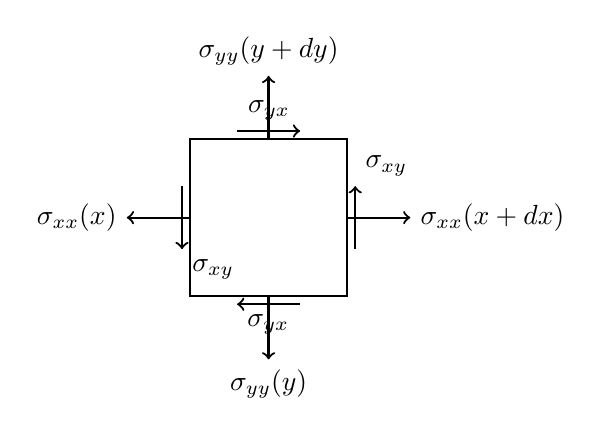
\begin{tikzpicture}
        % Draw the square
        \draw[thick] (-1,-1) rectangle (1,1);
        
        % Normal stresses
        \draw[->, thick] (-1,0) -- (-1.8,0) node[left] {$\sigma_{xx}(x)$};
        \draw[->, thick] (1,0) -- (1.8,0) node[right] {$\sigma_{xx}(x+dx)$};
        \draw[->, thick] (0,-1) -- (0,-1.8) node[below] {$\sigma_{yy}(y)$};
        \draw[->, thick] (0,1) -- (0,1.8) node[above] {$\sigma_{yy}(y+dy)$};
        
        % Shear stresses
        \draw[->, thick] (-.4,1.1) -- (0.4,1.1) node[above left] {$\sigma_{yx}$};
        \draw[->, thick] (.4,-1.1) -- (-0.4,-1.1) node[below right] {$\sigma_{yx}$};
        \draw[->, thick] (1.1,-.4) -- (1.1,.4) node[above right] {$\sigma_{xy}$};
        \draw[->, thick] (-1.1,.4) -- (-1.1,-.4) node[below right] {$\sigma_{xy}$};
        
    \end{tikzpicture}
    \caption{Stresses acting on an infinitesimal square at position $(x,y)$ with width $dx$ and height $dy$. For brevity, not all function arguments of $\fatsig$ are shown.}
    \label{fig:stress}
\end{figure}

Next consider the case of \textbf{pure shear}, where $\sigma_{xx}=\sigma_{yy}=0$. This case provides particular physical insight into shear stresses and the material's resistance to it.
Conservation of angular momentum requires that the sum of torques vanishes. Setting the lower left corner of the infinitesimal square to $x=y=0$, the only remaining torques originate from the upper and right sides, yielding
\begin{equation*}
\sum \mathbf{r}\times\mathbf{F}=dx\cdot (dy\cdot \sigma_{xy}) - dy\cdot (dx\cdot \sigma_{yx})=0.
\end{equation*}
Therefore, $\sigma_{xy}=\sigma_{yx}$, which already rules out certain oversimplified depictions of shear, such as those shown in Figure \ref{fig:shear}(A).

A useful intuition is that a material’s resistance to shear is equivalent to its ability to withstand diagonal loads. This can be illustrated by considering the strain along the diagonal $e_1$. The infinitesimal square is reinterpreted as an inner square subjected to diagonal forces, as depicted in Figure~\ref{fig:shear}(C). By distributing the shear forces along the square edges and resolving them into diagonal contributions, one obtains
\begin{align*}
dF_{11,x} &= \tfrac{1}{2}\,dx \cdot \sigma_{xy}, \\
dF_{11,y} &= \tfrac{1}{2}\,dy \cdot \sigma_{xy}, \\
dF_{11} &= \tfrac{1}{2}\,\sigma_{xy}\,\sqrt{dx^2+dy^2}.
\end{align*}
Assuming small shear angles, the resulting stress along the $e_1$ diagonal becomes
\begin{equation*}
\sigma_{11} = \frac{dF_{11}}{d_{11}}=\sigma_{xy},
\end{equation*}
with $d_{11}=\tfrac{1}{2}\sqrt{dx^2+dy^2}$. By symmetry, $\sigma_{22}=-\sigma_{xy}$, since the corresponding force can be calculated analogously but points inward rather than outward, resulting in the sign change.

Repeating the reasoning from the normal stress case, the strains along the diagonals are
\begin{align}
\label{eq}
\varepsilon_{11} &= \frac{\sigma_{11}}{E} - \nu \frac{\sigma_{22}}{E}, \\
\varepsilon_{22} &= \frac{\sigma_{22}}{E} - \nu \frac{\sigma_{11}}{E}.
\end{align}

Using $\sigma_{11}=-\sigma_{22}=\sigma_{xy}$ yields

\begin{align}
\sigma_{xy} &= \frac{E}{1+\nu}\,\varepsilon_{11}, \\
\sigma_{xy} &= -\frac{E}{1+\nu}\,\varepsilon_{22},
\label{eq:sigma_xy}
\end{align}
which shows that $\varepsilon_{11} = -\varepsilon_{22}$.

\begin{figure}
    \centering
    \begin{tikzpicture}
    %labels
    \node at (-3.5,2.5) {(A)};
    \node at (0.1,2.5) {(B)};
    \node at (5,2.5) {(C)};
    \node at (9,2.5) {(D)};
    %draw impossible case
    \coordinate (A1) at (-5,-1);
    \coordinate (B1) at (-3,-1);
    \coordinate (C1) at (-2.4,1);
    \coordinate (D1) at (-4.4,1);
    \coordinate (E1) at (-2.4,-1);
    \coordinate (F1) at (-5,1);
    \draw[-, thick] (A1) -- (B1) ;
        \draw[-, thick] (B1) -- (C1) ;
        \draw[-, thick] (C1) -- (D1) ;
        \draw[-, thick] (D1) -- (A1) ;
        \draw[dashed] (A1) -- (E1);
        \draw[dashed] (A1) -- (F1);
        % Draw the square
         \coordinate (A) at (-1,-1);
          \coordinate (B) at (1,-0.8);
          \coordinate (C) at (1.2,1.2);
          \coordinate (D) at (-0.8,1);
          \coordinate (E) at (2,-1);
          \coordinate (F) at (2,-0.7);
          \coordinate (Eup) at (-1,2);
          \coordinate (Fup) at (-0.7,2);
        \draw[-, thick] (A) -- (B) ;
        \draw[-, thick] (B) -- (C) ;
        \draw[-, thick] (C) -- (D) ;
        \draw[-, thick] (D) -- (A) ;
        \draw[dashed](A) -- (E) ;
        \draw[dashed](A) -- (F) ;
        \draw[dashed](A) -- (Eup);
        \draw[dashed](A) -- (Fup);
        \draw[dashed](A) -- (C) node[below left] {$e_1$};
        \draw[dashed](B) -- (D) node[below right] {$e_2$};
        \pic [draw, ->, angle radius=3cm, angle eccentricity=1.1, "$\theta$"] {angle = E--A--B};
        \pic [draw, <-, angle radius=3cm, angle eccentricity=1.1, "$\tilde{\theta}$"] {angle = Fup--A--Eup};

        
        % Shear stresses
        \draw[->, thick] (-.4,1.2) -- (0.6,1.3) node[above left] {$\sigma_{xy}$};
        \draw[->, thick] (.5,-1) -- (-0.5,-1.1) node[below right] {$\sigma_{xy}$};
        \draw[->, thick] (1.2,-.4) -- (1.3,.6) node[above right] {$\sigma_{xy}$};
        \draw[->, thick] (-1,.5) -- (-1.1,-.5) node[below right] {$\sigma_{xy}$};
        \pic [draw, ->, angle radius=3cm, angle eccentricity=1.1, "$\theta$"] {angle = E--A--B};




        % diagonal case

        % Draw the square
         \coordinate (A2) at (4,-1);
          \coordinate (B2) at (6,-0.8);
          \coordinate (C2) at (6.2,1.2);
          \coordinate (D2) at (4.2,1);
        \draw[dashed] (A2) -- (B2) ;
        \draw[dashed] (B2) -- (C2) ;
        \draw[dashed] (C2) -- (D2) ;
        \draw[dashed] (D2) -- (A2) ;


        % Draw inner square
         \coordinate (A3) at (5,-0.9);
          \coordinate (B3) at (6.1,0.2);
          \coordinate (C3) at (5.2,1.1);
          \coordinate (D3) at (4.1,0);
        \draw[-, thick] (A3) -- (B3) ;
        \draw[-, thick] (B3) -- (C3) node[midway, left, below] {$d_{11}$};
        \draw[-, thick] (C3) -- (D3) ;
        \draw[-, thick] (D3) -- (A3) ;

        \draw[->, thick] (5.7,0.7) -- (6.3,1.3) node[above left] {$\sigma_{11}$};
        \draw[->, thick] (4.45,-0.5) -- (3.9,-1.1) node[above left] {$\sigma_{11}$};
        \draw[->, thick] (4.55,0.55) -- (4,1.2) node[left] {$\sigma_{22}$};
        \draw[->, thick] (5.6,-0.4) -- (6.15,-0.95) node[right] {$\sigma_{22}$};
        %Forces
        \draw[->,thick] (8,-1) -- (10,-1) node[below] {$dF_{11,x}$};
        \draw[->,thick] (10,-1) -- (10,1) node[right] {$dF_{11,y}$};
        \draw[->,thick] (8,-1) -- (10,1) node[above left] {$dF_{11}$};
        
    \end{tikzpicture}
    \caption{(A) Shear stress is sometimes introduced in this form, with $\sigma_{yx}\neq 0$ and $\sigma_{xy}=0$. This configuration is not physically possible due to conservation of angular momentum. To reach such a deformation, one additionally requires a rigid body rotation. (B) Deformation in the case of pure shear. (C) Illustration of modeling the infinitesimal square as an inner square resisting diagonal loads. (D) Infinitesimal forces acting on the upper-right side of the inner square.}
    \label{fig:shear}
\end{figure}







With this, we have obtained the stress as a function of the strain, $\fatsig = \fatsig(\varepsilon_{xx}, \varepsilon_{yy}, \varepsilon_{11})$. Finally, we want to express the strain $\fateps$ as a function of the displacement $\fatu$.\\
We proceed in two partly redundant steps. First, we consider pure normal strain, which is intuitively straightforward. Subsequently, we derive an expression for $\fateps$ that explicitly describes shear strain. Note that the second part alone would already suffice; nevertheless, we include the first example because it provides a direct intuition for normal strain.\\
\textbf{Pure normal strain:} The bottom side of the outer square with side length $dx$ is elongated by $\partial u_x/\partial x\cdot dx$, yielding
\begin{equation*}
\varepsilon_{xx}=\frac{dx+\frac{\partial u_x}{\partial x}(x,y)\cdot dx-dx}{dx}=\frac{\partial u_x}{\partial x}(x,y).
\end{equation*}
Analogously, $\varepsilon_{yy}=\partial u_y/\partial y$.\\
What remains is to determine the dependence of the off-diagonal elements of $\fateps$ on $\fatu$.\\
\textbf{Shear strain:} For this purpose, we first perform a decomposition of the displacement gradient into symmetric and antisymmetric parts. Let $d\mathbf{r}$ denote the vector connecting two material points before deformation, and let $\fatu$ denote the displacement field. The vector connecting the same two material points in the deformed configuration is then
\begin{equation}
d\mathbf{r}'=(\mathbf{1}+\nabla\fatu )\cdot d\mathbf{r}.
\label{eq:nabla_u}
\end{equation}
From this, one can see that, roughly speaking, $\nabla\fatu$ is closely related to $\fateps$ since stretching a length $l_0$ by $\varepsilon$ yields $l=(1+\varepsilon)\, l_0$. As shown in \cite{fung2001classical}, one can decompose $\nabla \fatu$ into a deformation part $\fateps$ and a rigid body rotation $\mathbf{\omega}$:
\begin{equation*}
\nabla\fatu = \fateps + \mathbf{\omega},
\end{equation*}
with
\begin{equation}
\fateps=\frac{1}{2}\cdot (\nabla\fatu + \nabla\fatu^T)
\label{eq}
\end{equation}
being the symmetric part and $$\mathbf{\omega}=\frac{1}{2}\cdot (\nabla\fatu - \nabla\fatu^T)$$ the antisymmetric part of $\nabla\fatu$.\\
An intuitive interpretation is the following: Figure \ref{fig:shear} (B) shows an angle $\theta$. For small $\theta$, this angle is equal to the slope of the lower side of the square, such that $\theta=\partial u_y / \partial x$, and analogously $\tilde\theta=\partial u_x / \partial y$. We now consider two limiting cases:\\

Consider the case $\sigma_{xx}=\sigma_{yy}= 0$ and $\sigma_{xy}=\sigma_{yx}\neq 0$ without rigid body rotation. Intuitively, this causes a deformation of the square, as shown in Figure \ref{fig:shear} (B). Mathematically, this follows from $\omega_{xy}=1/2\, (\partial u_x/\partial y - \partial u_y / \partial x)=0$, implying $\partial u_y / \partial x=\partial u_x / \partial y$ and therefore $\theta=\tilde\theta$. Consequently, the angle in the lower-left corner of the square decreases from $\pi/2$. This changes the shape of the square, which the material resists, and therefore this contribution must be included in the solid mechanics equations. As discussed above, the material resistance to this deformation corresponds to a resistance to normal stress along the diagonal.\\
Consider the case of pure rigid body rotation with $\sigma_{xy}=0$. In this case, the lower side of the square rotates by $\theta$, while the left side rotates by the same angle in the same direction with $\theta=-\tilde{\theta}$ (note that $\tilde{\theta}$ is defined in the opposite direction of $\theta$, which explains the sign). Consequently, $\partial u_y / \partial x=-\partial u_x / \partial y$, such that $\nabla\fatu$ is antisymmetric. Since the shape of the square remains unchanged, the material does not resist this displacement, and therefore this contribution does not enter the solid mechanics equations.\\
Superposing these two cases yields the general case consisting of shear deformation and rigid body rotation. The above explains why only the symmetric part of $\nabla\fatu$ is used in the solid mechanics equation.\\

What remains is to relate $\varepsilon_{xy}$ to the strain along the diagonals $\varepsilon_{11}=-\varepsilon_{22}$. In the case of pure shear, we have $\varepsilon_{xx}=\varepsilon_{yy}=0$, such that
\begin{equation*}
\fateps =
\begin{pmatrix}
0 & \varepsilon_{xy} \\
\varepsilon_{xy} & 0
\end{pmatrix}
\end{equation*}
where the eigenvectors of $\fateps$ are trivially $(1,1)$ and $(-1,1)$. By equation \eqref{eq:nabla_u}, the diagonal of the infinitesimal rectangle is mapped to an elongated diagonal of identical orientation if and only if the diagonal directions coincide with the eigenvectors of $\fateps$. Therefore, $\varepsilon_{xy}$ can be related to the strain along the diagonal in the case of a square with $dx=dy$. In this case, the diagonal extends to

\begin{align*}
l_{e_1,d}&=\sqrt{(dx+\tilde\theta dy)^2+(dy+\theta dx)^2} \\
&=\sqrt{(dx\cdot(1+\theta))^2+(dy\cdot (1+\theta))^2} \\
&=(1+\theta)\cdot l_{e_1,i},
\end{align*}
where we have used $\theta=\tilde\theta$ since we consider pure shear. Finally, one obtains

\begin{align*}
\varepsilon_{xy}=\frac{1}{2}\left(\frac{\partial u_x}{\partial y}+\frac{\partial u_y}{\partial x}\right)=\frac{1}{2}\left(\tilde\theta+\theta\right)=\theta.
\end{align*}
The strain along the diagonal is then
\begin{equation*}
\varepsilon_{11}=\frac{l_{e_1,d}-l_{e_1,i}}{l_{e_1,i}}=\frac{(1+\theta)\cdot l_{e_1,i}-l_{e_1,i}}{l_{e_1,i}}=\theta,
\end{equation*}
so that $\varepsilon_{xy}=\varepsilon_{11}$. We have already derived the relation $\fatsig=\fatsig (\varepsilon_{11})$ in \eqref{eq:sigma_xy}; therefore, $\varepsilon_{11}$ can be replaced by $\varepsilon_{xy}$, yielding the final constitutive relation $\fatsig(\fatu)$:

\begin{align*}
\sigma_{xx}&=\frac{E}{1-\nu^2}(\varepsilon_{xx}+\varepsilon_{yy}\cdot \nu) \\
\sigma_{yy}&=\frac{E}{1-\nu^2}(\varepsilon_{yy}+\varepsilon_{xx}\cdot \nu) \\
\sigma_{xy}&=\frac{E}{1+\nu}\cdot \varepsilon_{xy}\\
\varepsilon_{xx}&=\frac{\partial u_x}{\partial x}\\
\varepsilon_{yy}&=\frac{\partial u_y}{\partial y}\\
\varepsilon_{xy}&=\frac{1}{2}\,\left(\frac{\partial u_x}{\partial y}+\frac{\partial u_y}{\partial x}\right).\\
\end{align*}


For FEM, the formulation of the consitiutive relation using Lame's parameters is more convenient. We define the Lame Parameters for 2D solid mechanics with
\begin{align*}
    \mu&:=\frac{E}{2\cdot(1+\nu)}\\
    \lambda&:=\frac{E\cdot \nu}{1-\nu^2}.
\end{align*}

With this we can rewrite the constitutive relation of the normal stresses to 
\begin{align*}
    \sigma_{xx}&=\frac{E}{1-\nu^2}(\varepsilon_{xx}+\varepsilon_{yy}\cdot \nu)\\
    &=\frac{E}{1-\nu^2}(\varepsilon_{xx}-\varepsilon_{xx}\cdot\nu+\varepsilon_{xx}\cdot \nu+\varepsilon_{yy}\cdot \nu)\\
    &=\frac{E}{1-\nu^2}(\varepsilon_{xx}\cdot(1-\nu)+tr(\fateps)\cdot \nu)\\
    &=\frac{E}{1+\nu}\varepsilon_{xx}+\frac{E\cdot \nu}{1-\nu^2}\cdot tr(\fateps)\\
    &=2\cdot \mu\cdot \varepsilon_{xx}+\lambda \cdot tr(\fateps)\\
\end{align*}
and analogously for $\sigma_{yy}$. The first Lame Parameter $\mu$ is easily found in the constitutive relation of $\sigma_{xy}$ and so we can now write the constitutive relation with respect to $\mu$ and $\lambda$ as
\begin{equation*}
    \fatsig = 2\cdot \mu\cdot \fateps + \lambda\cdot tr(\fateps).
\end{equation*}






Now that the constitutive relation has been established, we can proceed to the derivation of the PDE itself. The governing equation is essentially Newton’s second law, $F = m \cdot a$. Considering again an infinitesimal square element, the stresses described by $\fatsig$ give rise to a net force $\mathbf{F}$, which in turn would produce an acceleration $\mathbf{a}$ of the element. Since we are interested in the static case, we set $\mathbf{a} = \mathbf{0}$, and hence $\mathbf{F} = \mathbf{0}$. This condition already represents the desired PDE; what remains is to express $\mathbf{F}$ in terms of $\fatsig$.  

As illustrated in Figure \ref{fig:stress}, each side of the element is subject to normal and shear stresses. Each of these stresses contributes a force, and the sum of all forces must vanish. The force due to the stress $\sigma_{xx}(x)$, for example, is $\sigma_{xx}(x)\cdot dy$. Summing all contributions and setting the result to zero yields  

\begin{equation*}
    -\sigma_{xx}(x)\cdot dy + 
    \sigma_{xx}(x+dx)\cdot dy 
    - \sigma_{xy}(y)\cdot dx+ 
    \sigma_{xy}(y+dy)\cdot dx= 0
\end{equation*}
in the $x$-direction, and
\begin{equation*}
    -\sigma_{yy}(y)\cdot dx+
    \sigma_{yy}(y+dy)\cdot dx-
    \sigma_{xy}(x)\cdot dy+ 
    \sigma_{xy}(x+dx)\cdot dy= 0
\end{equation*}
in the $y$-direction.  

Dividing both equations by $dx \cdot dy$ and rewriting in vector form gives
\begin{equation}
    \left(
    \begin{matrix}
        (\sigma_{xx}(x+dx) - 
        \sigma_{xx}(x))/dx + 
        (\sigma_{xy}(y+dy) - 
        \sigma_{xy}(y))/dy\\
        
        (\sigma_{yy}(y+dy) -
        \sigma_{yy}(y))/dy +
        (\sigma_{xy}(x+dx) - 
        \sigma_{xy}(x))/dx
    \end{matrix}
    \right) = 
    \left(
    \begin{matrix}
        0\\
        0
    \end{matrix}
    \right).
\end{equation}

In the limit, only differential quotients remain, so that in compact notation
\begin{equation*}
    \left(
    \begin{matrix}
        \frac{\partial\sigma_{xx}}{\partial x} +
        \frac{\partial\sigma_{xy}}{\partial y}\\
        
        \frac{\partial\sigma_{yy}}{\partial y} +
        \frac{\partial\sigma_{xy}}{\partial x}
    \end{matrix}
    \right) = 
    \nabla\cdot \fatsig =
    \left(
    \begin{matrix}
        0\\
        0
    \end{matrix}
    \right),
\end{equation*}
which is the PDE sought.  

\textbf{Remark:} An additional intuition that emerges from this derivation is that, in static equilibrium, changes in the normal stresses must be counterbalanced by corresponding changes in the shear stresses in both the $x$- and $y$-directions. In the present model, these stress variations arise from discontinuities in the prestress.















\section{Derivation of the 2D Wave Equation}
\label{sec:derivation_wave}

For completeness, this section presents a derivation of the 2D wave equation on a membrane, complementing the previous derivation of the elasticity equation. The derivation follows the approach described in \cite{ClelandAndrewN2003Fon:}.  

As stated in section \ref{sec:assumptions}, the coupling between elasticity and the wave equation is introduced in a forward manner: the stress field $\fatsig \in \mathbb{R}^{2\times 2}$ obtained from the elasticity PDE is used as a coefficient function in the wave equation. The objective is to describe the displacement $u:\mathbb{R}^2 \rightarrow \mathbb{R}$ in the out-of-plane ($z$) direction.  

Once again, the derivation is based on Newton’s second law. Considering an infinitesimal square element, the in-plane stresses $\fatsig$ produce a net out-of-plane force $F$, leading to $F = m \cdot a \neq 0$.  

We begin with the normal stresses. Figure \ref{fig:wave_derivation_side} shows an infinitesimal square viewed along the $y$-axis. When the square is bent, the forces due to $\sigma_{xx}$ on the left and right sides no longer cancel, resulting in a net force. Although the total force is not generally aligned with the $z$-axis, the equilibrium condition from the elasticity PDE ensures that the in-plane force balance $\nabla \cdot \fatsig = \mathbf{0}$ is already satisfied. Consequently, only the $z$-component remains.  

The force contribution from $\sigma_{xx}(x)$ on the left side has slope $\partial u / \partial x(x)$, yielding a $z$-component
\[
dF_{x,l} = \frac{\partial u}{\partial x}(x)\, \sigma_{xx}(x)\, dy.
\]
Analogously, on the right side,
\[
dF_{x,r} = \frac{\partial u}{\partial x}(x+dx)\, \sigma_{xx}(x+dx)\, dy.
\]
Subtracting the two gives the net contribution from $\sigma_{xx}$:
\begin{align*}
    dF_x&=\frac{\partial u}{\partial x}(x+dx) \cdot \sigma_{xx}(x+dx)\cdot dy-\frac{\partial u}{\partial x}(x) \cdot \sigma_{xx}(x)\cdot dy\\
    &=\frac{\partial u}{\partial x}(x+dx) \cdot \left(\sigma_{xx}(x)+\frac{\partial\sigma_{xx}}{\partial x}(x)\cdot dx\right)\cdot dy-\frac{\partial u}{\partial x}(x) \cdot \sigma_{xx}(x)\cdot dy\\
    &=\sigma_{xx}(x)\cdot \frac{\partial^2u}{\partial x^2}\cdot dx\cdot dy+\frac{\partial u}{\partial x}(x+dx) \cdot\frac{\partial\sigma_{xx}}{\partial x}(x)\cdot dx\cdot dy\\
    &=\sigma_{xx}(x)\cdot \frac{\partial^2u}{\partial x^2}\cdot dx\cdot dy+\frac{\partial u}{\partial x}(x) \cdot\frac{\partial\sigma_{xx}}{\partial x} (x)\cdot dx\cdot dy+\frac{\partial^2u}{\partial x^2}(x) \cdot\frac{\partial\sigma_{xx}}{\partial x}(x)\cdot dx^2\cdot dy\\
    &\approx\sigma_{xx}(x)\cdot \frac{\partial^2u}{\partial x^2}\cdot dx\cdot dy+\frac{\partial u}{\partial x}(x) \cdot\frac{\partial\sigma_{xx}}{\partial x}(x)\cdot dx\cdot dy
\end{align*}
A similar calculation for $\sigma_{yy}$ gives
\[
dF_y \approx \sigma_{yy}(y)\, \frac{\partial^2 u}{\partial y^2}\, dx\, dy + \frac{\partial u}{\partial y}(y)\, \frac{\partial \sigma_{yy}}{\partial y}(y)\, dx\, dy.
\]

The shear stress components also contribute. Fixing $y$, the difference between $\sigma_{xy}(x,y)$ and $\sigma_{xy}(x+dx,y)$ produces a force proportional to the slope in the $y$-direction. Analogous to the calculation for $dF_x$, we obtain
\begin{align*}
    dF_{xy} &\approx \sigma_{xy}\, \frac{\partial^2 u}{\partial x \partial y}\, dx\, dy + \frac{\partial u}{\partial x}\, \frac{\partial \sigma_{xy}}{\partial y}\, dx\, dy,\\
    dF_{yx} &\approx \sigma_{xy}\, \frac{\partial^2 u}{\partial y \partial x}\, dx\, dy + \frac{\partial u}{\partial y}\, \frac{\partial \sigma_{xy}}{\partial x}\, dx\, dy.
\end{align*}

Summing all contributions, the total force on the element is
\begin{align*}
    dF &= \sigma_{xx}\, \frac{\partial^2 u}{\partial x^2}\, dx\, dy + \sigma_{yy}\, \frac{\partial^2 u}{\partial y^2}\, dx\, dy
    + \sigma_{xy}\, \frac{\partial^2 u}{\partial x \partial y}\, dx\, dy + \sigma_{xy}\, \frac{\partial^2 u}{\partial y \partial x}\, dx\, dy \\
    &\quad + \frac{\partial u}{\partial x}\, \frac{\partial \sigma_{xx}}{\partial x}\, dx\, dy + \frac{\partial u}{\partial y}\, \frac{\partial \sigma_{yy}}{\partial y}\, dx\, dy \\
    &\quad + \frac{\partial u}{\partial x}\, \frac{\partial \sigma_{xy}}{\partial y}\, dx\, dy + \frac{\partial u}{\partial y}\, \frac{\partial \sigma_{xy}}{\partial x}\, dx\, dy.
\end{align*}
The last four terms vanish due to $\nabla \cdot \fatsig = \mathbf{0}$, leaving
\[
dF = \nabla \cdot \left( \fatsig \cdot \nabla u \right)\, dx\, dy.
\]

With the element mass $dm = \rho\, dx\, dy$ (noting $\rho$ has units $\text{kg}/\text{m}^2$ in 2D) and acceleration $a = \partial^2 u/\partial t^2$, Newton’s second law $dF = dm \cdot a$ yields the governing PDE:
\begin{equation}
    \nabla \cdot \left( \fatsig \cdot \nabla u \right) = \rho \frac{\partial^2 u}{\partial t^2}.
\end{equation}















\begin{figure}
    \centering
    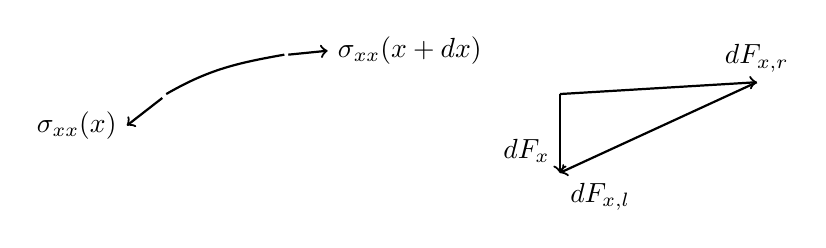
\begin{tikzpicture}
        % Draw bent shape (approximated by a curve)
        \draw[thick] (-1,0) to[out=30, in=190] (0.5,0.5);
        
        
        % Tangential stresses (sigma_xx) on both sides
        \draw[->, thick] (-1.05,-0.05) -- (-1.5,-0.4) node[left] {$\sigma_{xx}(x)$};
        \draw[->, thick] (0.55,0.5) -- (1.05,0.55) node[right] {$\sigma_{xx}(x+dx)$};
        
        %draw force vectors
        \coordinate (A) at (4,0);
        \coordinate (Ah) at (6.5,0);
        \coordinate (B) at (6.5,0.15);
        \coordinate (Bh) at (4,0.15);
        \coordinate (C) at (4,-1);
        \draw[->, thick] (A) -- (B) node[above] {$dF_{x,r}$};
        \draw[->, thick] (B) -- (C) node[below right] {$dF_{x,l}$};
        \draw[->, thick] (A) -- (C) node[above left] {$dF_x$};

        
    \end{tikzpicture}
    \caption{1D element under prestress showing tangential stresses causing a backward force in the wave equation.}
    \label{fig:wave_derivation_side}
\end{figure}
\clearpage



\chapter{Code}
\label{sec:appendixB}

This chapter presents the most relevant code fragments developed for this thesis.

\begin{minted}{python}
def make_geometry(p: Dict[str, Any]) -> SplineGeometry:
    """Construct the NGSolve/Netgen geometry from parameter dict ``p``."""
    geometry = SplineGeometry()
    # Boundaries (square domain)
    boundary_points = [(0.0, 0.0), (p["Lside"], 0.0), (p["Lside"], p["Lside"]), (0.0, p["Lside"])]
    pnums = [geometry.AppendPoint(*pt) for pt in boundary_points]
    # start-point, end-point, boundary-condition, domain on left side, domain on right side
    lines: List[Tuple[int, int, str, int, int]] = []
    for i in range(3):
        lines.append((pnums[i], pnums[i + 1], "fix", 1, 0))
    lines.append((pnums[3], pnums[0], "fix", 1, 0))
    # Electrodes
    w_el = p["el_width"]
    dists_from_middle = [-w_el / 2.0, +w_el / 2.0]

    for dist_from_middle in dists_from_middle:
        for lr in ("l", "r"):
            bc = ("left_" if lr == "l" else "right_") + ("inner" if dist_from_middle == (-w_el / 2.0) else "outer")
            pnts = points_on_parabola(p, dist_from_middle, lr)
            el_pnums: List[int] = [geometry.AppendPoint(*pt) for pt in pnts]
            for i in range(len(el_pnums) - 1):
                lines.append((el_pnums[i], el_pnums[i + 1], bc, 1, 1))

    # Perforated area
    perf_pts = points_on_circle(p, p["Rperf"], 0.0, p["h_elements_perf"],
                                p["Lside"] / 2.0, p["Lside"] / 2.0)
    perf_pnums: List[int] = [geometry.AppendPoint(*pt) for pt in perf_pts]
    for i in range(len(perf_pnums) - 1):
        lines.append((perf_pnums[i], perf_pnums[i + 1], "perf_border", 1, 1))
    if perf_pnums:
        lines.append((perf_pnums[-1], perf_pnums[0], "perf_border", 1, 1))

    # Drop masses with coffee ring
    for added_mass in p["added_masses"]:
        x_coord = added_mass["x_coord"]
        y_coord = added_mass["y_coord"]
        radius = added_mass["radius"]
        coffee_ring_width = added_mass["coffee_ring_width"]

        pnts_dic = {
            "inner": points_on_circle(p, radius - coffee_ring_width, 0.0,
                                      added_mass["h_elements_coffee"], x_coord, y_coord),
            "outer": points_on_circle(p, radius, 0.0,
                                      added_mass["h_elements_coffee"], x_coord, y_coord),
        }

        outer_nums = [geometry.AppendPoint(*pt) for pt in pnts_dic["outer"]]
        for i in range(len(outer_nums) - 1):
            lines.append((outer_nums[i], outer_nums[i + 1], "coffee_ring_outer", 1, 1))
        if outer_nums:
            lines.append((outer_nums[-1], outer_nums[0], "coffee_ring_outer", 1, 1))

        if coffee_ring_width > 0:
            inner_nums = [geometry.AppendPoint(*pt) for pt in pnts_dic["inner"]]
            for i in range(len(inner_nums) - 1):
                lines.append((inner_nums[i], inner_nums[i + 1], "coffee_ring_inner", 1, 1))
            if inner_nums:
                lines.append((inner_nums[-1], inner_nums[0], "coffee_ring_inner", 1, 1))

    # Add lines to geometry
    for p1, p2, bc, left, right in lines:
        geometry.Append(["line", p1, p2], bc=bc, leftdomain=left, rightdomain=right)

    return geometry

\end{minted}
\begin{minted}{python}
def generate_sig_fct(p: Dict[str, Any]) -> Any:
    """Principal stress tensor field as a diagonal ``CF``.

    Combines base membrane stress, electrode contributions, perforation scaling,
    and optional coffee-ring mass effects.
    """
    base_sig = p["sigsin"] * p["hsin"]
    el_add_sig = p["hcr"] * p["sigcr"] + p["hau"] * p["sigau"]

    sig_delta = 1 - p["sigpercentage_perf"]
    principal_sig = base_sig * (1 - sig_delta * geom_perf(p)) + el_add_sig * geom_el_both(p, x, y)

    for added_mass in p["added_masses"]:
        coffee_prestress = added_mass["coffee_prestress"]
        non_coffee_prestress = added_mass["non_coffee_prestress"]
        radius = added_mass["radius"]
        coffee_ring_width = added_mass["coffee_ring_width"]
        x_coord = added_mass["x_coord"]
        y_coord = added_mass["y_coord"]
        coffee_height = added_mass["coffee_height"]
        non_coffee_height = added_mass["non_coffee_height"]

        del_r = radius - coffee_ring_width
        step_inner = ceil((del_r - 2 * CF_EPS) - dist_circ(x_coord, y_coord, x, y))
        step_outer = ceil((radius + 2 * CF_EPS) - dist_circ(x_coord, y_coord, x, y))

        principal_sig += non_coffee_prestress * non_coffee_height * step_inner
        principal_sig += coffee_prestress * coffee_height * (step_outer - step_inner)

    sigfct = CF(((principal_sig, 0), (0, principal_sig)))
    return sigfct

\end{minted}
\clearpage
\begin{minted}{python}

def generate_rho_fct(p: Dict[str, Any]) -> Any:
    """Surface mass density field (``CF``) including electrodes and droplets."""
    rhofct = CF(0)

    if p.get("added_masses"):
        for added_mass in p["added_masses"]:
            eps = 2 * CF_EPS
            x_coord = added_mass["x_coord"]
            y_coord = added_mass["y_coord"]
            mass = added_mass["mass"]
            radius = added_mass["radius"]
            coffee_ring_width = added_mass["coffee_ring_width"]
            coffee_ring_perctg = added_mass["coffee_ring_perctg"]

            coffee_mass = mass * coffee_ring_perctg
            noncoffee_mass = mass - coffee_mass

            noncoffee_area = np.pi * (radius - coffee_ring_width) ** 2
            coffee_area = np.pi * radius ** 2 - noncoffee_area

            noncoffee_density = noncoffee_mass / noncoffee_area
            coffee_density = coffee_mass / coffee_area

            del_r = radius - coffee_ring_width
            step_inner = ceil((del_r - eps) - dist_circ(x_coord, y_coord, x, y))
            step_outer = ceil((radius + eps) - dist_circ(x_coord, y_coord, x, y))

            rhofct += noncoffee_density * step_inner
            rhofct += coffee_density * (step_outer - step_inner)

    rhofct += p["rhosin"] * p["hsin"] * (1 - (1 - p["mpercentage_perf"]) * geom_perf(p))
    rhofct += (p["hcr"] * p["rhocr"] + p["hau"] * p["rhoau"]) * (geom_el_both(p, x, y))

    return rhofct

\end{minted}
\clearpage
\begin{minted}{python}
def mode_detection(p, gfu, mesh):
    """Detect mode numbers from a grid function solution.

    Returns a string of the form "(nx, ny)".
    """
    gfnp = np_gridfct(p, gfu, mesh)
    gfnp_normed = gfnp / np.max(gfnp)
    row_sums = np.zeros(len(gfnp))
    col_sums = np.zeros(len(gfnp))

    for y_ind in range(len(gfnp)):
        row_sums[y_ind] = np.sum(gfnp_normed[:, y_ind])
    for x_ind in range(len(gfnp)):
        col_sums[x_ind] = np.sum(gfnp_normed[x_ind, :])

    n_maxs = [0, 0]
    for i, arr in enumerate([row_sums, col_sums]):
        maxs, _ = scipy.signal.find_peaks(arr, prominence=2)
        n_maxs[i] = len(maxs)

    return f"({n_maxs[1]},{n_maxs[0]})"
\end{minted}
\clearpage
\begin{minted}{python}
def stress(p, strain):
    """Return stress tensor for given strain based on parameter dict p."""
    E_fct = CF(p["Esin"] * (1 - (1 - p["Epercentage_perf"]) * geom_perf(p)))
    nu_fct = CF(p["nu"] * (1 - (1 - p["nupercentage_perf"]) * geom_perf(p)))
    mu_fct = CF(E_fct / (2 * (1 + nu_fct)))
    lam_fct = CF(E_fct * nu_fct / (1 - nu_fct * nu_fct))
    return 2 * mu_fct * strain + lam_fct * Trace(strain) * Id(2)

\end{minted}
\clearpage
\begin{minted}{python}
def force_CF(p, x, y):
    """Return coefficient functions for boundary forces (electrodes, coffee rings)."""
    abs_f = p["hcr"] * p["sigcr"] + p["hau"] * p["sigau"]
    dir_vec_len = sqrt(1 + (2 * p["a"] * y + p["b"]) ** 2)
    x_comp_l = 1.0 / dir_vec_len
    y_comp_l = -(2 * p["a"] * y + p["b"]) / dir_vec_len
    x_comp_r = -1.0 / dir_vec_len
    y_comp_r = -(2 * p["a"] * y + p["b"]) / dir_vec_len

    force_l = CF((abs_f * x_comp_l, abs_f * y_comp_l))
    force_r = CF((abs_f * x_comp_r, abs_f * y_comp_r))
    force_outer_coffee = CF((0, 0))
    force_inner_coffee = CF((0, 0))

    #only supports one coffee ring now. force_outer_coffee += for more than one.
    for added_mass in p["added_masses"]:
        abs_f_outer = added_mass["coffee_height"] * added_mass["coffee_prestress"]
        abs_f_inner = abs_f_outer - added_mass["non_coffee_height"] * added_mass["non_coffee_prestress"]
        dir_vec_len = dist_circ(added_mass["x_coord"], added_mass["y_coord"], x, y)
        x_comp = (x - added_mass["x_coord"]) / dir_vec_len
        y_comp = (y - added_mass["y_coord"]) / dir_vec_len
        force_outer_coffee = CF((abs_f_outer * x_comp, abs_f_outer * y_comp))
        force_inner_coffee = CF((abs_f_inner * x_comp, abs_f_inner * y_comp))

    return force_l, force_r, force_outer_coffee, force_inner_coffee
\end{minted}
\clearpage

\begin{minted}{python}
def generate_fes_ela(p, mesh):
    """Generate finite element space and assembled system for elasticity."""
    fes = VectorH1(mesh, order=3, dirichlet="fix")
    u = fes.TrialFunction()
    v = fes.TestFunction()
    gfu = GridFunction(fes)

    force_l, force_r, force_outer, force_inner = force_CF(p, x, y)
    f = LinearForm(
        force_l * v * ds("left_inner") - force_l * v * ds("left_outer")
        + force_r * v * ds("right_inner") - force_r * v * ds("right_outer")
        - force_outer * v * ds("coffee_ring_outer") + force_inner * v * ds("coffee_ring_inner")
    ).Assemble()

    a = BilinearForm(InnerProduct(stress(p, Sym(Grad(u))), Sym(Grad(v))).Compile() * dx)
    pre = Preconditioner(a, "bddc")
    a.Assemble()

    return fes, u, v, gfu, f, a, pre
\end{minted}
\clearpage
\begin{minted}{python}
def stress_field(p, gfuela, mesh):
    """Return combined stress field (elastic + prestress)."""
    sigfct = generate_sig_fct(p)
    fesstress = MatrixValued(L2(mesh, order=0), symmetric=True)
    ustress = GridFunction(fesstress)
    ustress.Interpolate(stress(p, Sym(Grad(gfuela))), fesstress)
    prestress = GridFunction(fesstress)
    prestress.Interpolate(sigfct, fesstress)
    return ustress + prestress
\end{minted}
\clearpage
\begin{minted}{python}
def generate_fes_wave(mesh, gfstress, rhofct, preconditioner: str = "multigrid"):
    """Generate FE spaces and assembled forms for wave problem."""
    feswave = H1(mesh, order=2, dirichlet="fix")
    u = feswave.TrialFunction()
    v = feswave.TestFunction()

    a = BilinearForm(feswave)
    a += SymbolicBFI(InnerProduct((gfstress * grad(u)), grad(v)))
    pre = Preconditioner(a, preconditioner)

    m = BilinearForm(feswave)
    m += SymbolicBFI(rhofct * u * v)

    a.Assemble()
    m.Assemble()

    return feswave, a, m, pre

\end{minted}
\clearpage
\begin{minted}{python}
def solve_pinvit(p, feswave, pre, a, m, verbose: bool = False):
    """Solve eigenvalue problem using block power iteration (PINVIT)."""
    num = p["num_modes"]
    u = GridFunction(feswave, multidim=num)
    r = u.vec.CreateVector()
    Av = u.vec.CreateVector()
    Mv = u.vec.CreateVector()
    freedofs = feswave.FreeDofs()
    vecs = [u.vec.CreateVector() for _ in range(2 * num)]

    # random initialization
    for vec in u.vecs:
        for i in range(len(u.vec)):
            vec.data[i] = np.random.rand() if freedofs[i] else 0

    asmall = Matrix(2 * num, 2 * num)
    msmall = Matrix(2 * num, 2 * num)
    lams = [1] * num
    oldlams = [1e12] * num
    num_iter = 0
    max_iter = 500
    while sum(abs(l - o) for l, o in zip(lams, oldlams)) > p["convcrit"] and num_iter < max_iter:
        num_iter += 1
        oldlams[:] = lams[:]
        for j in range(num):
            vecs[j].data = u.vecs[j]
            r.data = a.mat * vecs[j] - lams[j] * m.mat * vecs[j]
            vecs[num + j].data = pre.mat * r

        for j in range(2 * num):
            Av.data = a.mat * vecs[j]
            Mv.data = m.mat * vecs[j]
            for k in range(2 * num):
                asmall[j, k] = InnerProduct(Av, vecs[k])
                msmall[j, k] = InnerProduct(Mv, vecs[k])

        ev, evec = scipy.linalg.eigh(a=asmall, b=msmall)
        lams[:] = ev[:num]
        if verbose:
            print("Eigenvalues:", lams)

        for j in range(num):
            u.vecs[j][:] = 0.0
            for k in range(2 * num):
                u.vecs[j].data += float(evec[k, j]) * vecs[k]
    if num_iter > max_iter - 2:
        print("max iterations exceeded. return None.")
        return None, None
    return lams, u
\end{minted}
\clearpage
\begin{minted}{python}
def solve(p, freq_to_fit_to=None, mode_to_fit_to=None, ela: bool = True,
          preconditioner: str = "multigrid"):
    """Solve full simulation loop: elasticity + wave problem."""
    print("solving")
    mesh = generate_mesh(p)
    eigenvals = [0] * p["num_modes"]
    del_f = 10 * p["convcrit"]  # initialize to enter first iteration
    freq_fem = 0

    while abs(del_f) > p["convcrit"]:
        # elasticity
        gfuela = solve_ela(p, mesh)
        if ela:
            gfstress = stress_field(p, gfuela, mesh)
        else:
            sigfct = generate_sig_fct(p)
            fesstress = MatrixValued(L2(mesh, order=0), symmetric=True)
            prestress = GridFunction(fesstress)
            prestress.Interpolate(sigfct, fesstress)
            gfstress = prestress
        # wave
        feswave, eigenvals, multigfuwave = solve_wave(p, mesh, gfstress,
                                                      preconditioner=preconditioner)
        if not eigenvals:
            return None, None, None
        if freq_to_fit_to is None:
            del_f = 0
        else:
            results = result_dict(p, mesh, feswave, multigfuwave, eigenvals, include_modeshape=False)
            if mode_to_fit_to in results:
                freq_fem = results[mode_to_fit_to][0] * 1e3
            else:
                raise ValueError("Could not find mode_to_fit_to")
            del_f = freq_to_fit_to - freq_fem
            Pa_per_Hz = 1e3 * (p["Lside"] / 1e-3)  # empirical factor: 1 MPa -> 1 kHz per mm size
            if abs(del_f) > p["convcrit"]:
                p["sigsin"] += del_f * Pa_per_Hz
    return feswave, eigenvals, multigfuwave
\end{minted}